Ein Wagen fährt auf einer geraden Bahn. Eine Stroboskopaufnahme zeigt seinen Ort einmal pro Sekunde (die Punkte, darüber die Zeit):
\begin{center}
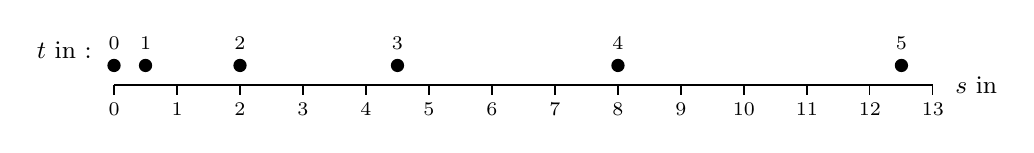
\begin{tikzpicture}[x=0.8cm, y=1cm]
 \draw[thick] (0,0) -- (13,0);
 \foreach \sk in {0,...,13} \draw (\sk,0) -- (\sk,-0.12);
 \foreach \sk in {0,1,...,13} \node[below, font=\scriptsize] at (\sk,-0.1) {$\sk$};
 \fill[black] (0,0.25) circle (2.4pt);
 \fill[black] (0.5,0.25) circle (2.4pt);
 \fill[black] (2,0.25) circle (2.4pt);
 \fill[black] (4.5,0.25) circle (2.4pt);
 \fill[black] (8,0.25) circle (2.4pt);
 \fill[black] (12.5,0.25) circle (2.4pt);
 \node[above, font=\scriptsize] at (0,0.33) {$0$};
 \node[above, font=\scriptsize] at (0.5,0.33) {$1$};
 \node[above, font=\scriptsize] at (2,0.33) {$2$};
 \node[above, font=\scriptsize] at (4.5,0.33) {$3$};
 \node[above, font=\scriptsize] at (8,0.33) {$4$};
 \node[above, font=\scriptsize] at (12.5,0.33) {$5$};
 \node[right, font=\small] at (13.2,0) {$s$ in \si{\meter}};
 \node[left, font=\small] at (-0.2,0.45) {$t$ in \si{\second}:};
\end{tikzpicture}
\end{center}
\begin{abcliste}
\abc Stellen Sie eine Tabelle $t$ -- $s$ auf und skizzieren Sie das $s(t)$-Diagramm.
\abc Jonas verbindet im $s(t)$-Diagramm den ersten Punkt $(0\,|\,0)$ und den letzten Punkt $(5\,|\,12.5)$ mit einer Geraden, „weil der Wagen ja vom einen zum anderen Ort fährt“. Welche Bewegung würde seine Gerade beschreiben, und warum stimmt sie nicht?
\end{abcliste}
